\chapter{Mini tutorial de LaTeX}\label{ChapTutorial}

[Este capítulo es un tutorial breve: cada sección muestra un recurso
básico de LaTeX con un ejemplo que compila. Borre este capítulo cuando su
tesis esté lista, o consérvelo como referencia. Lo que aquí se ejemplifica
—listas, ecuaciones, letras griegas, citas, figuras y tablas— es lo que
más se usa al escribir una tesis.]

\section{Estructura: capítulos, secciones y referencias cruzadas}

Un documento se divide en \verb|\chapter|, \verb|\section| y
\verb|\subsection|. Para referirse a otra parte del documento se pone una
etiqueta con \verb|\label| y se cita con \verb|\ref|. Por ejemplo, este
capítulo es el capítulo~\ref{ChapTutorial}, y la
sección~\ref{sec:ecuaciones} trata de ecuaciones. Las notas al pie se
hacen con \verb|\footnote|, como esta.\footnote{Esto es una nota al pie
de ejemplo. Sirve para aclaraciones que no caben en el texto principal.}

\section{Listas}

Hay tres tipos de lista. La lista sin orden usa \verb|itemize|:

\begin{itemize}
\item Primer elemento de la lista.
\item Segundo elemento de la lista.
\item Tercer elemento de la lista.
\end{itemize}

La lista numerada usa \verb|enumerate|:

\begin{enumerate}
\item Primer paso del procedimiento.
\item Segundo paso del procedimiento.
\item Tercer paso del procedimiento.
\end{enumerate}

La lista de descripción usa \verb|description|:

\begin{description}
\item[Concepto] Descripción breve del concepto.
\item[Método] Descripción breve del método.
\end{description}

\section{Ecuaciones}\label{sec:ecuaciones}

Una ecuación en línea se escribe entre signos de dólar: la energía es
$E = mc^2$, donde $E$ es la energía, $m$ es la masa y $c$ es la velocidad
de la luz. Una ecuación centrada y numerada usa el entorno
\verb|equation|:

\begin{equation}
E = mc^2
\label{eq:energia}
\end{equation}

donde $E$ es la energía, $m$ es la masa y $c$ es la velocidad de la luz.
La ecuación~\eqref{eq:energia} se cita con \verb|\eqref|. Para varias
ecuaciones alineadas por el signo igual se usa \verb|align| (del paquete
\verb|amsmath|, ya cargado por la clase):

\begin{align}
a^2 + b^2 &= c^2 \\
x &= \frac{-b \pm \sqrt{b^2 - 4ac}}{2a}
\label{eq:cuadratica}
\end{align}

donde $a$, $b$ y $c$ son coeficientes constantes. La
ecuación~\eqref{eq:cuadratica} es la fórmula general de segundo grado.

\section{Letras griegas}

Las letras griegas se escriben en modo matemático con su nombre en
inglés precedido de una barra invertida. La tabla~\ref{tab:griegas}
muestra las más usadas.

\begin{table}[htbp]
\centering
\caption[Letras griegas de ejemplo]{Letras griegas más usadas.}
\label{tab:griegas}
\begin{tabular}{lll}
\toprule
Nombre & Minúscula & Mayúscula \\
\midrule
alfa & $\alpha$ & --- \\
beta & $\beta$ & --- \\
gamma & $\gamma$ & $\Gamma$ \\
delta & $\delta$ & $\Delta$ \\
pi & $\pi$ & $\Pi$ \\
omega & $\omega$ & $\Omega$ \\
lambda & $\lambda$ & $\Lambda$ \\
mu & $\mu$ & --- \\
sigma & $\sigma$ & $\Sigma$ \\
\bottomrule
\end{tabular}
\end{table}

Por ejemplo, la constante $\pi$ vale aproximadamente $3.1416$, y un
incremento se escribe $\Delta x$. Las mayúsculas que coinciden con el
alfabeto latino (como la A de alfa) no tienen comando propio: se escriben
directamente.

\section{Citas bibliográficas}

Las referencias se guardan en el archivo \verb|.bib| y se citan con
\verb|\cite|. Por ejemplo, para un libro se escribe
\verb|\cite{libro-ejemplo}|, que produce \cite{libro-ejemplo}; para un
artículo, \verb|\cite{articulo-ejemplo}|, que produce
\cite{articulo-ejemplo}; y para un sitio web,
\verb|\cite{sitio-ejemplo}|, que produce \cite{sitio-ejemplo}. Con
\verb|natbib| (ya cargado por la plantilla) también se puede citar el
autor en el texto con \verb|\citet{libro-ejemplo}|:
\citet{libro-ejemplo} es un libro de ejemplo. Al final del documento, el
comando \verb|\bibliography| genera la lista con el estilo elegido en
\verb|\bibliographystyle|.

\section{Figuras}

Una figura se incluye con \verb|\includegraphics| dentro de un entorno
\verb|figure|, siempre con pie (\verb|\caption|) y etiqueta
(\verb|\label|) para citarla en el texto. La
figura~\ref{fig:escudo-ejemplo} muestra cómo incluir una imagen externa.

\begin{figure}[htbp]
\centering
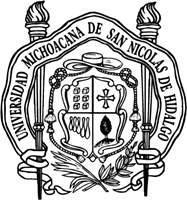
\includegraphics[width=0.25\textwidth]{Latex/Classes/Escudos/UMSNH_BN}
\caption[Ejemplo de imagen externa]{Ejemplo de imagen externa: escudo
de la UMSNH incluido con \texttt{\textbackslash includegraphics}.}
\label{fig:escudo-ejemplo}
\end{figure}

También se pueden dibujar figuras directamente en LaTeX con TikZ, como
la parábola del capítulo~\ref{Chap2}. El ancho se controla con
\verb|width|: \verb|0.25\textwidth| es un cuarto del ancho del texto.

\section{Tablas}

Una tabla se hace con el entorno \verb|tabular| dentro de \verb|table|,
con pie y etiqueta, igual que las figuras. Para tablas con mejor aspecto
se usa el paquete \verb|booktabs|, con las reglas \verb|\toprule|,
\verb|\midrule| y \verb|\bottomrule| en lugar de \verb|\hline| (véase la
tabla~\ref{tab:griegas}). La tabla~\ref{tab:ejemplo} del
capítulo~\ref{Chap2} muestra la versión sencilla con \verb|\hline|.

\section{Cómo compilar}

La forma recomendada es \verb|latexmk|, que repite las pasadas
necesarias (incluida la bibliografía) automáticamente:

\begin{verbatim}
latexmk -pdf plantilla-tesis-umsnh.tex
\end{verbatim}

Sin \verb|latexmk|, a mano (tres pasadas de \verb|pdflatex| con
\verb|bibtex| en medio):

\begin{verbatim}
pdflatex plantilla-tesis-umsnh.tex
bibtex plantilla-tesis-umsnh
pdflatex plantilla-tesis-umsnh.tex
pdflatex plantilla-tesis-umsnh.tex
\end{verbatim}

El PDF resultante no se versiona: se genera al compilar. Para limpiar
los archivos intermedios, use \verb|latexmk -c|.
